\chapter{相关研究综述}
\label{chap:related_work}

本章主要介绍本课题的相关研究和实践工作,
其中包括使用专业设备的多视角高精度3D重建方法,
基于少量非受限环境照片的高效3D人脸重建方法,
可微分渲染以及它在人脸重建中的应用。

\section{基于非受限环境照片的高效3D人脸重建}

除上述这些力求准确的方法外,还有一些方法则希望降低采集的设备成本和复杂度,从而推动3D人脸重建技术在更多领域的应用。
这些方法通常建立在上述高精度方法的基础上,通过采集大量人脸的数据,从中学习并建立更多的关于人脸的先验知识,从而大大降低解空间的维度。
得益于此,甚至可以实现从单张非受限环境中拍摄的照片中重建3D人脸。
但相对应地,这些方法重建的结果可能缺失高频信息,或者产生逼真但不准确的结果。

3D可形变模型(3DMM)是这类方法中的先驱者,且这类模型在如今也仍然被广泛使用。
最初\citet{3DMM}利用200个激光扫描的人脸模型,包括人脸的几何和材质,然后认为新的人脸模型可以通过对这些模型进行线性组合来得到。
并且作者将不同人之间的差异通过主成分分析获取其中最重要的部分。
然后作者使用可微分渲染的方法,将该模型与采集到的新的照片进行匹配,并同时估计环境光照的参数,从而实现了从单张照片中重建3D人脸。
该方法仍需要人工指定一个较为准确的初始化。
\citet{deep3d}用已有的人脸关键点识别算法代替人工初始化,并使用可微分渲染来从大量人脸照片中训练神经网络,该网络可实现输入一张照片,直接输出3DMM人脸模型的参数。其最大优势在于,虽然使用神经网络,但无需使用昂贵的大量高精度3D数据进行训练。
DECA\citep{DECA}则在重建FLAME模型的基础上,额外添加了表情相关的动态细节。
\citet{ZielonkaBT22}利用人脸识别算法提取的特征,试图降低人脸远近和大小间的歧义,重建物理尺度更准确的3D人脸模型。
此外,该作者也使用了可微分渲染来捕获输入中的表情,弥补人脸识别对表情的不敏感。
\citet{1022667848.nh,feng2018prn}则选择了不输出3DMM模型的参数,而是直接输出3D人脸模型的顶点坐标。
还有很多方法\citep{GarridoVWT13,CaoBZB15,ShiWTC14,IchimBP15}也是使用类似的思路从单目照片或视频中重建3D人脸,并通过图像中的线索为3DMM模型添加更多细节,使其更加逼真。
\citet{SchonbornEFV15}与本文第\ref{chap:method}章中希望解决的问题类似,希望逆渲染任务能更加适应未知背景的条件,但该作者的思路是对背景应用一个较为通用的模型,且采用的是非基于梯度的方法。
本文将在现有计算可见性梯度的方法的基础上,提出一种无需为背景建模的,适应未知背景的梯度计算方法。

以上方法的输入均是在非受限环境下拍摄的照片,其环境光照信息是未知的。
但在实验室的受控环境下,也有一些方法通过数据建立更多的先验知识从而减少所需采集的数据量。
\citet{MekaHPZFFKYBDDB19}通过图片到图片的神经网络,输入两张RGB梯度照明的照片,生成稠密的反射场,从而实现了任意光照条件下的渲染。但该方法作为2D方法,无法简单地扩展到任意视角的3D渲染。且神经网络的输出虽然看上去非常逼真,但在物理上可能不够准确。
\citet{ZhangZZLCYXY22}使用多个VAE分别对采集到的人脸的表情、几何形状、纹理进行解耦、编码和生成,从而实现高效地编辑、驱动所捕获的高精度人脸模型。

\section{可微分渲染}

可微分渲染旨在求解渲染得到的图像关于渲染参数的梯度,以解决逆渲染问题,即从渲染结果的图像中恢复渲染该图像所需的参数。
前述的很多3D人脸重建方法都使用到了可微分渲染相关的技术作为其合成分析方法的一部分,但其运用还很初级。
例如,现有方法均只对每个像素的着色过程计算了梯度,而忽略了几何遮挡等因素。
本文也试图推进更现代的可微分渲染在3D人脸重建中的应用。
下文将介绍通用的可微分渲染领域的一些研究。

\paragraph{基于光线追踪的可微分渲染}
这类方法通过光线追踪的方法,通过蒙特卡洛采样,模拟大量光线在场景中的传播,无偏地估计每个像素的颜色,同时计算该过程的梯度。
这类方法通常计算量较大,且由于随即采样,其估计的梯度具有一定噪声。
\citet{redner}提出了一种使用蒙特卡洛光线追踪的可微分的基于物理的渲染方法,其具有正确的可见性梯度。
Mitsuba 2\citep{Mitsuba2}是一个多功能的渲染框架,可以用于解决各种渲染问题。
它创新性地使用了一种重参数化技术来计算几何遮挡相关的梯度。
\citet{ZeltnerSGJ21}提出将渲染过程和求微分过程的采样解耦,从而降低梯度估计的噪声。

\paragraph{基于光栅化的可微分渲染}
第二类可微分渲染旨在提高性能,以支持合成分析中迭代优化中所需的大量迭代次数。
这类方法基于实时渲染中使用的光栅化渲染方法。
他们主要针对解决形状或姿态估计等任务,它们使用局部信息渲染和着色3D网格,而不考虑全局光照。
这类方法的难点依然是如个计算几何遮挡相关的可见性梯度。
\citet{softras}将每个三角形光栅化为具有可配置模糊半径的概率云,这些云根据其他可配置参数进行启发式组合。这种模糊使覆盖率成为关于顶点位置的连续函数,这对于获得可见性梯度是必要的。
但是,模糊也意味着不透明表面在边缘周围变得透明,从而导致图像不正确。因此需要人工调整这些参数以在图像正确性和梯度质量之间达到平衡。
DIB-R\citep{ChenLGSLJF19}输出一个额外的alpha通道,该通道通过可配置的模糊半径扩展到覆盖像素之外。该alpha通道可用于近似可见性梯度,但仅当参考图像也有alpha遮罩时才能使用。
此外,位于其他几何体前面的轮廓也无法获得可见性梯度。
其模糊半径的参数也需要人工调整。
\citet{KatoUH18}在反向传播过程中基于几何信息在三角形边缘上近似出基于图像的梯度。但是,这些梯度与渲染的图像不一致。
\citet{nvdiffrast}提出了一个模块化的渲染器,其中抗锯齿模块可产生可见性梯度,但它需要处于边缘的三角形正好被渲染到了图像中,否则其产生的梯度就较为稀疏,给优化带来偏差。
\citet{ColeGSVZ21}提出了一种在离散的光栅化算法的基础上解算可见性梯度的方法。该方法也会引入少量模糊。
\citet{LyuHL0TT21}使用球作为代理,为渲染加上了近似的阴影。以更好地拟合目标图像。

\section{基于物理的高质量人脸3D渲染}

若要通过逆渲染的方法,基于可微分渲染重建3D人脸,首先需要一个高质量的3D人脸材质模型和渲染器。
本节将简要介绍计算机图形学业内常用的人脸3D渲染技术。

\paragraph{基于物理的渲染}

在早期的实时3D渲染中,由于计算性能的限制,模型的着色通常是基于一些简单的经验公式的。
而如今,基于物理的渲染(PBR)已经成为了主流,其渲染效果更加逼近真实世界的光照效果。
在基于物理的渲染中,材质模型通常表征了材质的一些物理属性,使其可以直接从现实中测量得到。其渲染方式也是对物理过程更加真实的近似。
这也给从照片进行逆渲染奠定了基础。

其中当前应用较为广泛的模型之一是迪士尼提出的Disney BSDF模型\citep{PBR_disney}。该模型可广泛用于描述生活中的绝大多数材质,包括金属、塑料、玻璃、橡胶、布等。
该模型由迪士尼应用于自己电影的离线渲染中,后被Blender、Unreal Engine等渲染器借鉴。
该模型的参数包括:
基础颜色,表征了材质对不同波长的光的反射率;
金属度,表征了材质是金属或电介质;
粗糙度,表征了材质表面的粗糙程度;
镜面反射,取决于物体的折射率;
以及其他一些共十余个参数。
这些参数也即在3D重建中所需求解的参数。

\paragraph{次表面散射}
除了上述参数外,次表面散射效果在人脸上较为明显,且其渲染较为复杂,因此在此单独介绍。次表面散射是指光线在入射物体之后,在其表面附近多次散射,再从与入射不同的位置出射的现象。

迪士尼介绍了其在离线渲染中使用的模型\citep{SSS_disney},这是对物理模型的蒙特卡洛模拟数据的数值近似。在离线渲染中,也会直接使用光线追踪对散射现象进行模拟,以达到更逼真的效果。
屏幕空间次表面散射\citep{SSSSS}在实时渲染中应用较广,其直接重用了原本渲染所需计算的数据,从而减小了开销。
纹理空间次表面散射\citep{texSSS}的提出较早,其基本思路是将会发生散射的光线先渲染在纹理空间,然后对其进行多次高斯模糊和叠加,从而计算散射效果。
\citet{SpSSS}提出牺牲一定的角对称性,以提升模糊的计算效率。
Unity3D在其渲染器中也使用了屏幕空间算法\citep{SSS_u3d},但其实现是基于\citet{SSS_disney}的模型进行随机采样,而非使用高斯模糊近似。

目前离线渲染大多使用光线追踪进行模拟,而实时渲染则使用屏幕空间次表面散射。
但对于多视角3D重建来说,纹理空间的方法或许更加合适,其计算的结果可以被多个视角共享。

\begin{figure}
    \centering
    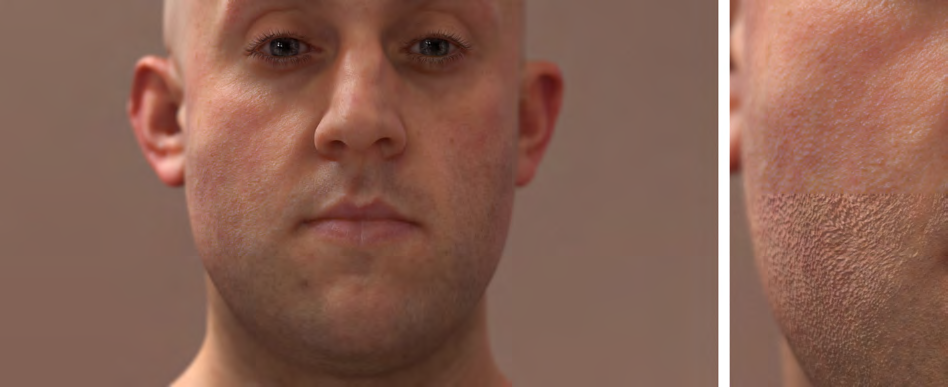
\includegraphics[width=\linewidth]{figures/sss}
    \caption[次表面散射人脸渲染效果]
    {次表面散射人脸渲染效果\citep{SpSSS}。
    在应用次表面散射之前(右下)和之后(右上)的近距离比较。}
\end{figure}

\paragraph{基于图像的光照}

除了对物理本身的建模外,对物体所处环境的准确建模也是逼真渲染的重要一环。
在早期的实时渲染中,通常使用简单的环境光照,点光源,方向光源等解析模型。
但这些模型并不能准确建模采集摄影中使用的柔光箱等设备产生的光照效果。

近年来,基于图像的光照(IBL)技术得到了广泛的应用,其基本思路是将环境光照建模为一个环境贴图,大大提升了光照建模的精度。
\citet{unreal_ssa}介绍了在Unreal Engine中所使用的分离求和近似,使环境贴图作为照明的渲染可以达到实时的效率。
